\documentclass[12pt]{article}
\usepackage[colorlinks,breaklinks,linkcolor=red,citecolor=blue]
{hyperref} 
\usepackage{graphicx,multicol,mdwlist}
\def\itemautorefname~#1\null{(#1)\null}
\usepackage{charter,amsmath,amssymb,breakurl}
\usepackage{eulervm}
\usepackage[letterpaper,margin=1in]{geometry}
\title{Math 265 Quiz 4 Solutions}\author{}\date{}
\let\cos\relax\DeclareMathOperator{\cos}{\mathsf{cos}}
\let\sin\relax\DeclareMathOperator{\sin}{\mathsf{sin}}
\let\ln\relax\DeclareMathOperator{\ln}{\mathsf{ln}}
\everymath{\displaystyle}
\begin{document}
\maketitle
\thispagestyle{empty}

\begin{multicols}{2}
Consider the vector field $\mathbold{F}\left(x,y\right)
=\left\langle 3y,-3x\right\rangle$, which is shown
at the right, together with the curve $C$,
which consists of a semicircle centered at the origin
between $\left(-1,1\right)$ and $\left(1,-1\right)$,
joined to a line segment with the same endpoints.
$C$ is oriented counterclockwise.
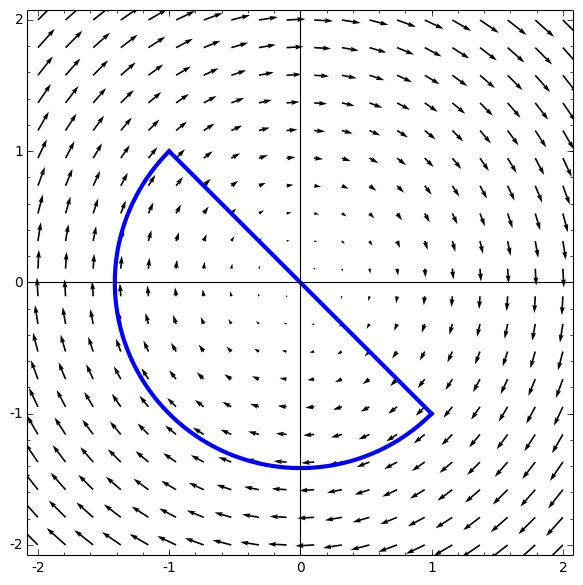
\includegraphics[scale=.6]{Cardioid}
\end{multicols}

\begin{enumerate}
\item\label{First} Is $\mathbold{F}$ conservative?\\
{\bf Solution.}
No, since $\mathsf{curl}\left(\mathbold{F}\right)
=Q_x-P_y=-6\ne 0$.
\item Calculate the circulation $\oint_C\mathbold{F}
\cdot d\mathbold{r}$ directly.\\
{\bf Solution.}
\begin{itemize}
\item Put $\mathbold{r}_1\left(t\right)=\sqrt{2}
\left\langle \cos{t},\sin{t}\right\rangle$
with $\frac{3\pi}{4}
\le t\le\frac{7\pi}{4}$.
\item $\mathbold{F}\left(\mathbold{r}_1\left(t\right)\right)
=3\sqrt{2}
\left\langle \sin{t},-\cos{t}\right\rangle$
\item $\mathbold{r}'_1\left(t\right)
=\sqrt{2}\left\langle -\sin{t},\cos{t}\right\rangle$
\item $\mathbold{F}\left(\mathbold{r}_1\left(t\right)\right)
\cdot\mathbold{r}'_1\left(t\right)
=6\left(-\sin^2{t}-\cos^2{t}\right)=-6$
\item $\oint_{C_1}\mathbold{F} \cdot d\mathbold{r}
=\int_{3\pi/4}^{7\pi/4}-6\;dt=-6\pi$
\item Put $\mathbold{r}_2\left(t\right)=
\left\langle -t,t\right\rangle$ with $-1\le t\le 1$
\item $\mathbold{F}\left(\mathbold{r}_2\left(t\right)\right)
=3\left\langle t,t\right\rangle$
\item $\mathbold{r}'_2\left(t\right)
=\left\langle -1,1\right\rangle$
\item $\mathbold{F}\left(\mathbold{r}_2\left(t\right)\right)
\cdot\mathbold{r}'_2\left(t\right)=0$
\item $\oint_{C_2}\mathbold{F} \cdot d\mathbold{r}=0$
\item So $\oint_C\mathbold{F} \cdot d\mathbold{r}=-6\pi$
\end{itemize}
\item Calculate the circulation $\oint_C\mathbold{F}
\cdot d\mathbold{r}$ using Green's Theorem.\\
{\bf Solution.}
$\mathsf{curl}\left(\mathbold{F}\right)=-6$ by
\autoref{First}, so
\[\int_R-6\;dA=\int_{3\pi/4}^{7\pi/4}\int_0^{\sqrt{2}}-6r
\;drd\theta
=-3\left.\int_{3\pi/4}^{7\pi/4}r^2\right|_0^{\sqrt{2}}\;d\theta
=-6\int_{3\pi/4}^{7\pi/4}d\theta=-6\pi.\]

\item Calculate the outward flux $\oint_C\mathbold{F}
\cdot\mathbold{n}\;ds$ using Green's Theorem.\\
{\bf Solution.}
$P_x+Q_y=0$ so
$\oint_C\mathbold{F}
\cdot\mathbold{n}\;ds=\int_R0\;dA=0$.
\end{enumerate}
\end{document}
